\documentclass[12pt]{ctexart}
\usepackage{fancyhdr} 
\usepackage[normalem]{ulem} 
\usepackage{soul}
\usepackage{soulutf8} 
\usepackage{xcolor}
\usepackage{amsmath} 
\usepackage{graphicx}
\usepackage{epstopdf}%图片插入
\usepackage[hidelinks]{hyperref}%目录设置

\sethlcolor{yellow}
\fancyfoot[C]{\thepage}	
\pagestyle{fancy}
\fancyhead{}

\renewcommand{\thesection}{第\chinese{section}章}
\renewcommand{\thesubsection}{\arabic{section}.\arabic{subsection}}
\newcommand{\mathcolorbox}[2]{\colorbox{#1}{$ #2$}}
\numberwithin{equation}{subsection}


\title{\Huge{统计物理}}
\author{Harichane}
\begin{document}

\maketitle
\thispagestyle{empty}%删除本页页码
\newpage

\tableofcontents
\addcontentsline{toc}{section}{目录}
%\thispagestyle{empty}%删除目录页码
\setcounter{page}{1}
\setcounter{section}{5} 
\newpage%分页

\section{统计物理的基本概念}
	\setcounter{subsection}{1} %将小节数从2开始
	\subsection{微观状态的经典描写与量子描写}
  	\subsubsection{ 子系:}
  		组成系统的基本单元,可以是气体中的分子等,也可以代表某一个自由度等.目前可以简单地理解成粒子。
	\subsubsection{ 相空间:}
		若系统由$N$个子系构成,每个子系的自由度为$r$,整个系统的自由度为$s=Nr$,则需要$2s$个广义坐标和广义动量${q_1}, \cdots ,{q_s},{p_1}, \cdots ,{p_s}$,用这$2s$个坐标和动量构成的空间称为\textbf{相空间}(或$\Gamma$ 空间),相空间中的一个点就代表系统的一个微观状态。
	\subsubsection{ 相体元:}
		相空间中的小体积元$d\Omega$。
		\[d\Omega  = d{q_1} \cdots d{q_s}d{p_1} \cdots d{p_s}\]
  	\subsubsection{Free Particle}
  		自由粒子的能量:
		\begin{equation}
			\varepsilon  = \frac{1}{{2m}}\left( {p_x^2 + p_y^2 + p_z^2} \right) = \frac{{{p^2}}}{{2m}}\
		\end{equation}
	\subsubsection{One-dimensional harmonic oscillator}
		一维谐振子的能量:
		\begin{equation}
			\varepsilon  = \frac{{{p^2}}}{{2m}} + \frac{1}{2}m{\omega ^2}{x^2}
		\end{equation}
	\subsubsection{ 边长为L的正方形容器中的自由粒子的能量(量子描写):}
		\begin{equation}
			\varepsilon  = \frac{1}{{2m}}\left( {p_x^2 + p_y^2 + p_z^2} \right) = \frac{{2{\pi ^2}{\hbar ^2}}}{{m{L^2}}}\left( {n_1^2 + n_2^2 + n_3^3} \right)
		\end{equation}
	\subsubsection{ 量子态:}
		例如${n_1} = 1,{n_2} = 1,{n_3} =  - 1$的态(简记为(1,1,-1))的能量为${\varepsilon _{1,1, - 1}} = \frac{{2{\pi ^2}{\hbar ^2}}}{{m{L^2}}} \times 3 = {\varepsilon _0}$,为最低能级。
	\subsubsection{ 简并度\texorpdfstring{$g$}.:}
		属于统一能级不同量子态数称为该能级的简并度。例如,上例中的${\varepsilon _0}$有$2^3=8$个不同的量子态,记为$g_0=8$.
	\subsubsection{ 一维谐振子的能量(量子描写):}
		\begin{equation}
			{\varepsilon _0} = \left( {n + \frac{1}{2}} \right)h\upsilon ,n = 0,1,2, \cdots 
		\end{equation}
		
		一维谐振子每一能级只有一个量子态,即简并度$g_n=1$.
	\subsubsection{ 子相体积:}
		在\colorbox{yellow!100}{经典极限条件下},对量子态的求和可以 代替为对子相空间的积分.
		\centerline{\footnotesize 子系的一个量子态$\longleftrightarrow$大小为$h^r$ 的子相体积}
	\subsubsection{ 全同性原理:}
		\textbf{全同粒子}是指他们的内禀性质(如质量、电荷、自旋等)完全相同;

		\textbf{全同性原理}:\textbf{全同粒子的交换不引起新的系统的量子态},或者说\textbf{全同粒子是不可分割的.}
	\subsubsection{ \textbf{全同粒子系统}波函数的对称性:}
		当交换任何两个粒子的全部坐标(位置,自旋)时,全同粒子系统的波函数只允许两种情况:或者波函数不变(波函数对称),或者波函数变号(波函数反对称)
	\subsubsection{ 费米子和玻色子:}
		\textbf{玻色子:}自旋为$s\hbar(s=0,1,2,\cdot)$的粒子,如光子$(s=1)$,$\pi$介子$(s=0)$ 等.其波函数是\textbf{交换对称}的,遵从\textbf{玻色-爱因斯坦统计};

		\textbf{费米子:}自旋为$\hbar$的半奇整数倍$(s=1/2,3/2,\cdot)$的粒子,如所有的轻子(电子,$\tau$子,$\mu$子),质子,中子(以上均为$s=1/2$)等,波函数是\textbf{交换反对称的},遵从\textbf{费米-狄拉克统计};

		\textbf{复合粒子:}如果是由偶数个费米子或玻色子构成,则为玻色子;由奇数个费米子组成,则为费米子.

	\subsubsection{ 泡利不相容原理:}
		全同费米子系统,不允许有两个全同的费米子处于同一个单粒子量子态;

		全同玻色子系统热一个单粒子态上占据的粒子数是不受限制的.
	\subsubsection{ 定域子系:}
		对于全同多粒子系统,若各个粒子的波函数被局限在空间不同的范围内没有重叠,则可以从粒子所处的不同的位置区分它们,这种子系称为\textbf{定域子系};与此相反的子系则称为\textbf{非定域子系}.
		\begin{figure}[htbp]
			\centering%图片居中
			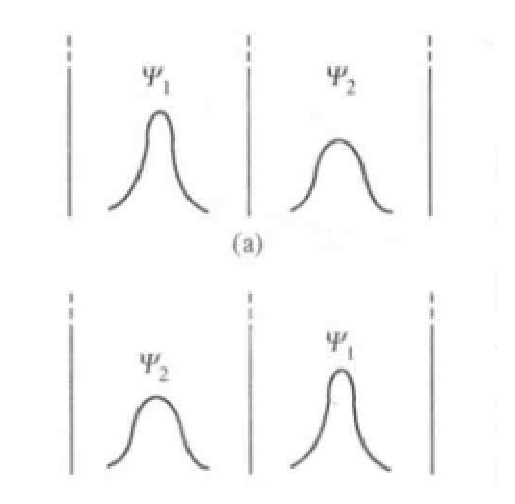
\includegraphics[scale=1]{1.eps}
			\caption{定域子系}
		\label{定域子系}
		\end{figure}
	\subsubsection{ 子系的量子态与(全同多粒子)系统的量子态:}
		设子系有3个不同的量子态,系统有2个粒子.

		对于定域子系:每一个粒子有3个量子态可选择,则2个粒子的量子态的组合有$3^2=9$个不同的量子态.

		对于非定域玻色子,由于粒子不可分辨,则组合数为${\text{C}}_3^1 + {\text{C}}_3^1=6$;

		对于非定域费米子,由于不能有两个费米子处于同一量子态,则组合数为${\text{C}}_3^1=3$;

	\subsubsection{ 等几率原理:}
	处于平衡态下的孤立系,系统各个可能的微观状态出现的几率相等.可能的微观状态指的是给定$(E,V,N)$的系统的可能的微观状态. 	
\section{近独立子系组成的系统}
\subsection{分布与系统的微观态\ 最可几分布}
	\subsubsection{ 近独立子系:}
		组成系统的粒子之间的相互作用可以忽略不计,即系统的总能量$E$等于各个粒子能量之和.由于粒子之间完全没有相互作用,粒子之间不可能交换能量,系统就不可能达到平衡态并保持平衡.

	\subsubsection{ 粒子按能级的分布\texorpdfstring{$a_\lambda$}.:}
		粒子的能级从低到高排序:${\varepsilon _1},{\varepsilon _2}, \cdots ,{\varepsilon _\lambda }, \cdots $,相应的各个能级的\textbf{简并度}为${g_1},{g_2}, \cdots ,{g_\lambda }, \cdots $,令${a_1},{a_2}, \cdots ,{a_\lambda }, \cdots $ 代表这些能级上占据的粒子数,称为粒子按能级的\textbf{微观分布},简记为{$a_\lambda$},不同的{$a_\lambda$}代表不同的微观分布.

		在固定的$(E,V,N)$的宏观状态下,允许出现的微观分布必须满足:
		\begin{equation}
			\sum\limits_\lambda  {{a_\lambda }}  = N\label{7.1.1}
		\end{equation}
		\begin{equation}
			\sum\limits_\lambda  {{\varepsilon _\lambda }{a_\lambda }}  = E\label{7.1.2}
		\end{equation}
\subsection{定域子系\ 麦克斯韦-玻尔兹曼分布}
	\subsubsection{ 分布\texorpdfstring{$a_\lambda$}.对应的\textbf{系统微观状态数}\texorpdfstring{$W(\{a_\lambda\})$}.:}
	\subsubsection{ 最可几分布\ 平均分布:}
		最可几分布即一定宏观状态下所有可能出现的微观分布中,出现几率最大的分布;

		若最可几分布出现的几率远大于其他分布,那么最可几分布等于平均分布.
	\subsubsection{ 麦克斯韦-玻尔兹曼分布(MB分布):}
		全同定域子系的最可几分布$\{a_\lambda\}$所对应的系统量子态数$W(\{a_\lambda\})$为:
		\begin{equation}
		W\left( {\{ {a_\lambda }\} } \right) = \frac{{N!}}{{\prod\limits_\lambda  {{a_\lambda }!} }}\prod\limits_\lambda  {g_\lambda ^{{a_\lambda }}} 
		\end{equation}

		最可几分布为:
		\begin{equation}
		{\tilde a_\lambda } = {g_\lambda }{e^{ - \alpha  - \beta {\varepsilon _\lambda }}}\label{7.1.4}
		\end{equation}

		即为\textbf{麦克斯韦-玻尔兹曼分布}.

		可以证明最可几分布是尖锐成峰的极大,故满足\hl{${\tilde a_\lambda } = {\bar a_\lambda }$}
	\subsubsection{ MB分布中参数\texorpdfstring{$\alpha$}.与\texorpdfstring{$\beta$}.的确定:}
		引入\textbf{子系配分函数$Z$}:
		\begin{equation}
			\mathcolorbox{yellow}{Z \equiv \sum\limits_\lambda  {{g_\lambda }{e^{ - \beta {\varepsilon _\lambda }}}} \label{7.1.5}}
		\end{equation}

		将(\ref{7.1.4})和(\ref{7.1.1})分别代入(\ref{7.1.1})和(\ref{7.1.2}),得:
		\begin{gather}
			\mathcolorbox{yellow}{\alpha= \ln \frac{Z}{N}}\\
			\mathcolorbox{yellow}{E=-N\frac{\partial }{{\partial \beta }}\ln Z}
		\end{gather}


% 加粗
%\textbf{}

% 斜体
%\textit{}

% 下划线
%\underline{}

% 删除线
%\sout{}

% 高亮
%\hl{}
%\colorbox{yellow!100}{边长为L的正方形容器中的自由粒子}

%\begin{equation}

%\end{equation}
\end{document}
